\documentclass[10pt,a4paper]{article}
\usepackage{geometry}
 \geometry{
 a4paper,
 total={170mm,257mm},
 left=20mm,
 top=20mm,
 }
\usepackage[spanish]{babel}
\usepackage[utf8]{inputenc}
\usepackage{graphicx}
\usepackage{wrapfig}
\usepackage{amssymb, amsmath}
\usepackage{tikz}
\usetikzlibrary{decorations.pathreplacing}
\newcommand{\tikzmark}[1]{\tikz[overlay,remember picture] \node[baseline] (#1) {};}
\tikzset{My Node Style/.style={midway, right, xshift=3.0ex, align=left, font=\small, draw=none, thin, text=black}}
\newcommand\VerticalBrace[4][]{%
    % #1 = draw options
    % #2 = top mark
    % #2 = bottom mark
    % #4 = label
\begin{tikzpicture}[overlay,remember picture]
  \draw[decorate,decoration={brace, amplitude=1.5ex}, #1] 
    ([yshift=1ex]#2.north east)  -- ([yshift=-1ex]#3.south east)
        node[My Node Style] {#4};
\end{tikzpicture}
}
\setlength{\parindent}{0cm}
\title{Resumen puesta a tierra de apoyos}
\author{MakerGarage}
\date{Abril 2021}

\begin{document}

\maketitle
\begin{center}
    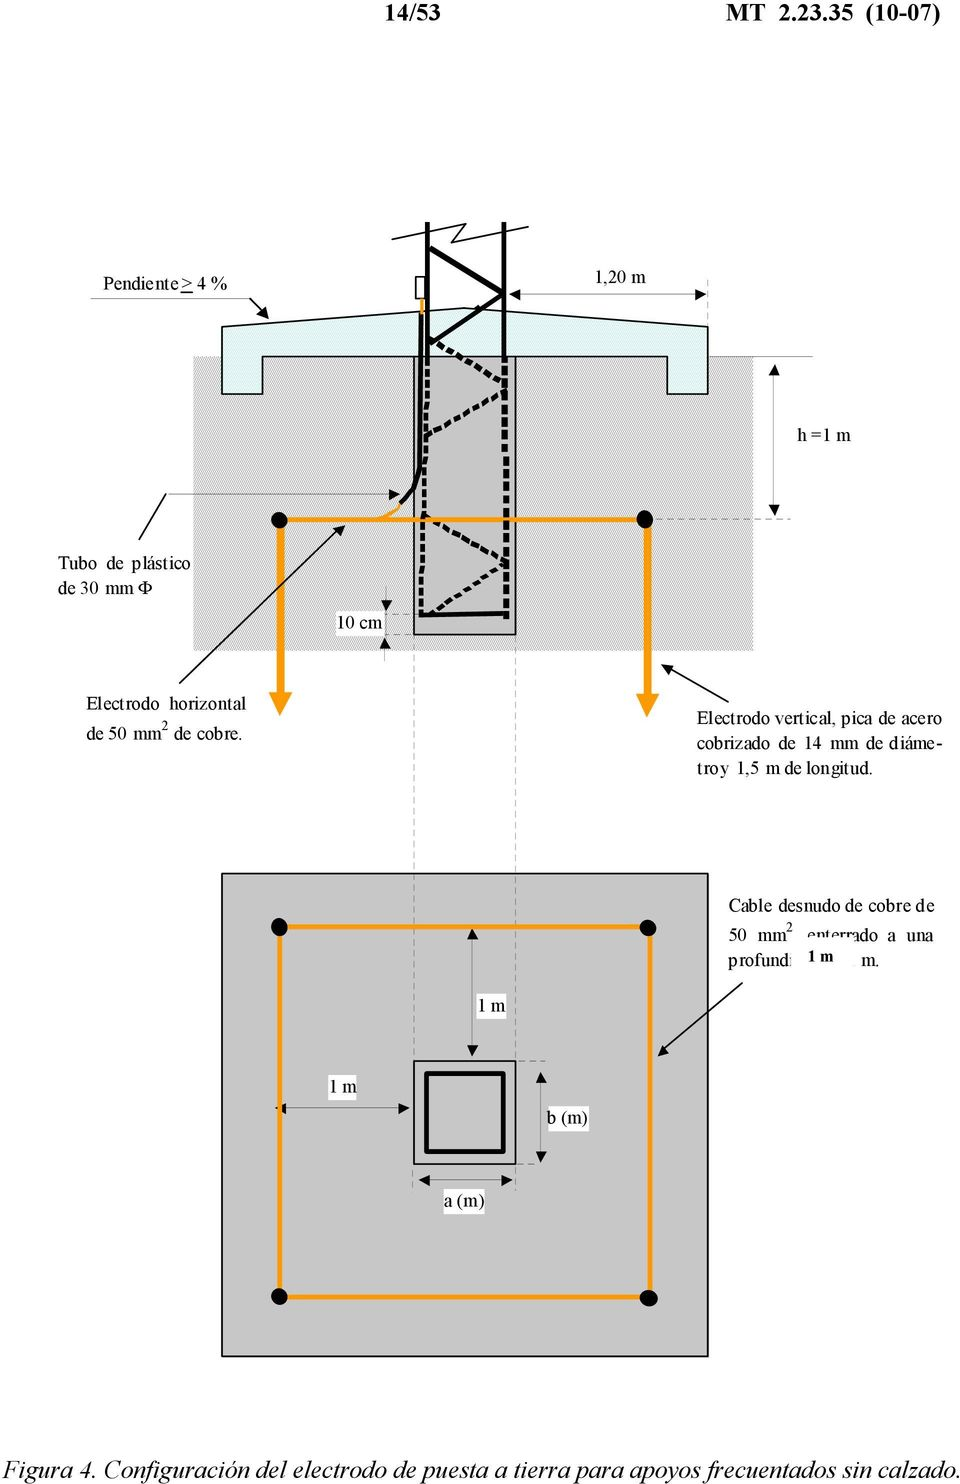
\includegraphics[trim = {0cm 1cm 0cm 1cm},clip,scale = 1.6]{assets/page_15.jpg}
\end{center}
\newpage

\section{Pasos a seguir}
$Z_{1A}$ Impedancia secuencia directa de la subestación A \\
$Z_{2A}$ Impedancia secuencia inversa de la subestación A \\
$Z_{0A}$ Impedancia secuencia homopolar de la subestación A \\
$Z_{EA}$ Impedancia a tierra de la subestación A \\
$Z_{1L}$ Impedancia directa de la línea \\
$Z_{2L}$ Impedancia inversa de la línea \\
$Z_{WL}$  \\
$Z_{WW0}$ \\


En este tipo de problemas buscamos calcular la intensidad de defecto que circula por nuestra pica de tierra $I_T$, una vez tengamos conocido este valor procedemos a comprobar si cumple los criterios que iremos viendo a continuación.
\\

Cabe destacar que podemos distinguir varias categorías:
\begin{itemize}
    \item $3^a$ Categoría (Alimentada por 1 subestación y sin cable de tierra)\tikzmark{top 1}
    
    \item $2^a$ Categoría (Alimentada por 1 subestación y sin cable de tierra)\tikzmark{bottom 1}
    
    \item $2^a$ Categoría (Alimentada por 2 subestaciones y sin cable de tierra)\,\rightarrow\, $I_E = I_{F1} + I_{F2}$
    
    \item $2^a$ Categoría (Alimentada por 2 subestaciones y con cable de tierra)
\end{itemize}
\VerticalBrace[ultra thin, black]{top 1}{bottom 1}{$I_E = I_F$}

Una vez hemos conseguido calcular la $I_E$ que circula por nuestro electrodo de puesta a tierra tenemos que comprobar que cumple siguiendo el siguiente esquema.

\begin{enumerate}
    \item Comprobamos que $V_E < 2 \cdot V_C$\tikzmark{top 1}
    \begin{itemize}
        \item[]
        \item[] \hspace{0.7cm}\Downarrow\, $No\,cumplimos$
        \item[] \hspace{1cm}
    \end{itemize}
    \item Comprobamos que $V_C' < V_C$ \hspace{0.325cm}\tikzmark{bottom 1}
    \begin{itemize}
        \item[]
        \item[] \hspace{0.7cm}\Downarrow\, $No\,cumplimos\,(Aplicamos\,\,medidas\,\,adicionales)$
        \item[] \hspace{1cm}
    \end{itemize}
    
    \item Comprobamos que $V_P' < V_P$\, y\, $V_{P_{acceso}}' < V_{P_{acceso}}$

\end{enumerate}
\VerticalBrace[ultra thin, black]{top 1}{bottom 1}{Tensiones de contacto}

Diferencias a la hora de calcular la $I_E$ en función del circuito:
\begin{itemize}
    \item $3^a$ Categoría (Alimentada por 1 subestación y sin cable de tierra)
            \begin{itemize}
                \item Neutro conectado
                $$
                \left|I_{F}\right| \simeq \frac{c \cdot U_{n}}{\sqrt{3} \cdot \sqrt{X_{n}^{2}+\left(R_{n}+R\right)^{2}}}
                $$
                c = 1'1 \\
                $U_n$ = Tensión de la línea \\
                R = Resistencia de puesta a tierra del apoyo \\
                $X_n$ = Impedancia del neutro \\
                $R_n$ = Resistencia del neutro
                
                \item Neutro aislado
                $$
                \left|I_{F}\right|=\frac{\sqrt{3} \cdot c \cdot U_{n} \cdot\left(\omega \cdot C_{a}\cdot 10^{-6} \cdot L_{a}+\omega \cdot C_{c}\cdot 10^{-6} \cdot L_{c}\right)}{\sqrt{1+\left(\omega \cdot C_{a}\cdot 10^{-6} \cdot L_{a}+\omega \cdot C_{c}\cdot 10^{-6} \cdot L_{c}\right)^{2} \cdot(3 R)^{2}}}
                $$
                c = 1'1 \\
                $U_n$ = Tensión de la línea \\
                R = Resistencia de puesta a tierra del apoyo \\
                $C_a$ = Capacidad de las líneas aéreas = 0'006 \mu F/Km \\
                $C_c$ = Capacidad de las líneas subterráneas = 0'25 \mu  F/Km \\
                $L_a$ = Longitud de las líneas aéreas en km \\
                $L_c$ = Longitud de las líneas subterráneas en km
            \end{itemize}   
    
    \item $2^a$ Categoría (Alimentada por 1 subestación y sin cable de tierra)
        \\
        
        Se calcula igual que una de $3^a$ Categoría (Alimentada por 1 subestación y sin cable de tierra)
        
    \newpage
    \item $2^a$ Categoría (Alimentada por 2 subestaciones y sin cable de tierra)
    $$
    I_{F1}+I_{F2} = I_E =\frac{\sqrt{3} \cdot c \cdot \vec{U}_{n}}{2 \cdot \vec{Z}_{1}+\vec{Z}_{0, s c t}+3 \cdot R}
    $$
    
    $$
    \vec{Z}_{1}=\vec{Z}_{2}=\frac{1}{\frac{1}{\vec{Z}_{1A}+\vec{Z}_{1 L} \cdot l_{a}}+\frac{1}{\vec{Z}_{1B}+\vec{Z}_{1 L} \cdot l_{b}}}
    $$
    
    $$
    \vec{Z}_{0, s c t}=\frac{1}{\frac{1}{3 \cdot \vec{Z}_{E A}+\vec{Z}_{0 A}+\vec{Z}_{0 L, s c t} \cdot l_{a}}+\frac{1}{3 \cdot \vec{Z}_{E B}+\vec{Z}_{0 B}+\vec{Z}_{0 L, s c t} \cdot l_{b}}}
    $$
    \item $2^a$ Categoría (Alimentada por 2 subestaciones y con cable de tierra)
    \\
    
    En este caso tenemos una parte de la corriente que se va a disipar por nuestro apoyo $I_T$ y por los apoyos colindantes $I_A + I_B$ y el resto de la corriente retorna a la subestación $(1 - r)\cdot3\cdot I_{OA}$ 
    \begin{center}
        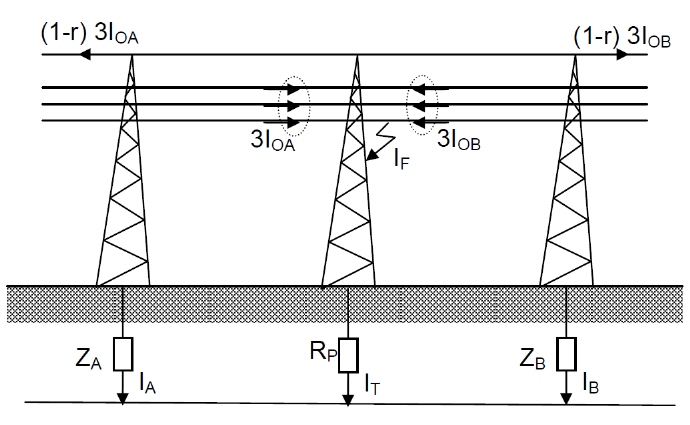
\includegraphics[scale = 0.6]{assets/100.png}
    \end{center}
    En este caso tenemos que $I_E = I_A + I_B + I_T$ siendo $I_T$ la corriente que queremos obtener, los pasos a seguir son los siguientes:
    \begin{enumerate}
        \item Saco $I_F$ la cual depende de $Z_1$ y $Z_0$
        $$
        \vec{I}_{F}=\frac{\sqrt{3} \cdot c \cdot \vec{U}_{n}}{2 \cdot \vec{Z}_{1}+\vec{Z}_{0}}
        $$
        
        c = 1'1 \\
        $\vec{U}_{n}$ = Tensión de la línea en Voltios
        
        
        $$
        \vec{Z}_{1}=\vec{Z}_{2}=\frac{1}{\frac{1}{\vec{Z}_{1A}+\vec{Z}_{1 L} \cdot l_{a}}+\frac{1}{\vec{Z}_{1B}+\vec{Z}_{1 L} \cdot l_{b}}}
        $$
        
        $Z_A$ = Impedancia de la subestación A \xleftarrow[]{}Dato\\ 
        $Z_B$ = Impedancia de la subestación B \xleftarrow[]{}Dato\\ 
        $Z_{1L}$ = Impedancia directa \\
        $l_a$ = Longitud del apoyo hasta la subestación A [km] \\
        $l_b$ = Longitud del apoyo hasta la subestación B [km]
        
        $$
        \vec{Z}_{0}=\frac{1}{\frac{1}{\vec{Z}_{0 A}+\vec{Z}_{0 L} \cdot l_{a}}+\frac{1}{\vec{Z}_{0 B}+\vec{Z}_{0 L} \cdot l_{b}}}
        $$
        
        $Z_{0A}$ = Impedancia homopolar de la subestación A \\
        $Z_{0B}$ = Impedancia homopolar de la subestación B \\
        $Z_{0L}$ = Impedancia homopolar del CT con cable de tierra \\
        $l_a$ = Longitud del apoyo hasta la subestación A \\
        $l_b$ = Longitud del apoyo hasta la subestación B
        \item Calculo r (factor de reducción) el cual depende de $Z_{WL}$ y $Z_{ww0}$ que a su vez dependen de $\delta$ y de r nos quedamos con el módulo
        
        $$
        \vec{r}=1-\frac{\vec{Z}_{W L}}{\vec{Z}_{w w 0}}
        $$
        
        $$
        \vec{Z}_{W L}=
         \left[
        \omega \cdot \frac{\mu_{0}}{8}+j \cdot \omega \cdot \frac{\mu_{0}}{2 \cdot \pi} \cdot \ln \frac{\delta}{D_{W L}}
        \right] \cdot 10^3 \, [\frac{\Omega}{km}]
        $$
        
        $w$ = $2 \cdot \pi \cdot 50$ \\
        $\mu_{0}$ = Permeabilidad del vacio = $4 \cdot \pi \cdot 10^{-7}$ \\
        $D_{W L}$ = Distancia media geométrica entre el cable de tierra y conductores [m]
        
        $$
        \vec{Z}_{w w 0}=\frac{R_{w}}{n}+\left[ \omega \cdot \frac{\mu_{0}}{8}+j \cdot \omega \cdot \frac{\mu_{0}}{2 \cdot \pi} \cdot\left[\ln \frac{\delta}{r_{w w}}+\frac{\mu_{r}}{4 \cdot n}\right]\right]\cdot 10^3
        \, [\frac{\Omega}{km}]
        $$
        
        $\mu_{0}$ = Permeabilidad en el vacío = $4 \cdot \pi \cdot 10^{-7}$ \\
        $r_{w w}$ = Radio equivalente de los cables de tierra (debe de ir en metros) (diámetro/2) \\
        n = Número de cables de tierra \\
        $R_w$ = Resistencia por unidad de longitud del cable de tierra $R_w = \frac{\rho_w}{S}$ \\
        
        $$
        \delta=\frac{1,85}{\sqrt{\frac{\omega \cdot \mu_{0}}{\rho}}} \,[m]
        $$
        
        $\rho$ densidad del terreno en $\frac{\omega}{m}$\\
        $\delta$ = Profundidad media de las lineas de intensidad de corriente que retornan por el terreno \\
        $\mu_{0} = 4\pi\cdot10^-7$ Permeabilidad en el vacío
        
        Una vez tengo $I_F$ y r puedo calcular $I_E$
        $$I_E = \left|\vec{r}\right| \cdot \left|\vec{I_F}\right|$$
        
        \item Saco $Z_A$ y $Z_B$ y con ellas saco $Z_E$
        \\
        
        Es importante destacar que $Z_A$ y $Z_B$ se refieren a la impedancia de los apoyos a un lado y otro del apoyo de estudio, son diferentes a las $Z_A$ y $Z_B$ que empleamos para sacar \vec{$Z_1$} las cuales se refieren a la impedancia de la subestación correspondiente.
        $$
        Z_{E}=\frac{Z_{A} * Z_{B}}{Z_{A}+Z_{B}}
        $$
        
        $$
        Z_{A}=Z_{B}=\frac{1}{2}\left(Z_{S}+\sqrt{Z_{S} \cdot\left(4 \cdot R_{t}+Z_{S}\right)}\right)
        $$
        
        $R_t$ = Resistencia de los apoyos colindantes
        
        $$
        Z_{S}=\vec{Z}_{w w 0} \cdot a_{m}
        $$
        
        $a_{m}$ longitud media de los vanos en km \\
        $\vec{Z}_{w w 0}$ calculada antes
        \\
        
        Es importante recordar que la raiz de un vector se calcula como:
        $$\sqrt{\vec{Z_s}} = \sqrt{\left | \vec{Z_s} \right |} \angle \frac{ángulo}{2}$$
    
    \newpage
    \item Por ultimo calculo la $I_T$
    \begin{center}
        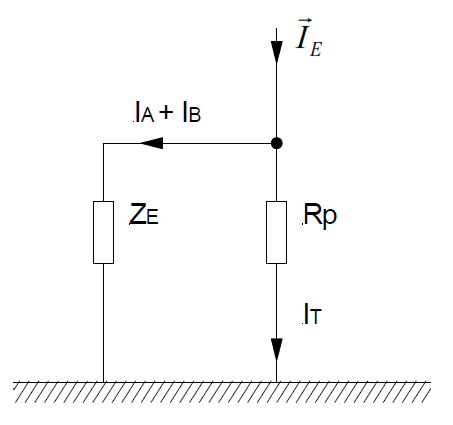
\includegraphics[scale = 0.45]{assets/102.png}
    \end{center}
    Para calcular $R_p$ tenemos que elegir un electrodo (UNESA) o una pica y calcularlo como $R_p = K_r \cdot \rho$
    $$
    \vec{Z}_{\text {total }}=\frac{\vec{Z}_{E} \cdot R_{p}}{\vec{Z}_{E}+R_{p}} \quad
    $$
    
    $$
    \vec{U}_{E}=\vec{Z}_{\text {total }} \cdot \vec{I}_{E} \quad 
    $$
    
    $$
    \vec{U}_{E}=\vec{Z}_{\text {total }} \cdot \vec{r} \cdot \vec{I}_{F}
    $$
    
    $$
    I_T =\frac{U_E}{R_p}
    $$
    \end{enumerate}
\end{itemize}
\newpage
\section{Apoyo no frecuentado 3 categoría}
Nos encontramos en una línea de 3 categoría por tanto no disponemos de conductor de tierra.
\\
Al ser apoyo no frecuentado, solamente debe cumplir que las protecciones actúen
Pasos a seguir:
\begin{itemize}
    \item Calcular la resistencia del electrodo 
    \item Calcular la intensidad de defecto 
    \item Calcular el tiempo de desconexión 
\end{itemize}
\\
Comenzamos:
\begin{itemize}
    \item Calcular la resistencia del electrodo \\
        \begin{itemize}
            \item En el caso de ser una sola pica \\
        $$R = \frac{\rho}{L}$$
        $\rho = Resistividad\,\,del\,\,terreno\,\,[\Omega \cdot m]$
        $L$ = Longitud de la pica [m]
        \\
        
        \item En el caso de ser un electrodo (UNESA)
        \begin{itemize}
            \item $K_r$ \hspace{1.5cm} \tikzmark{top 1}
            \item $K_p$
            \item $K_c = K_{p_{acceso}}$ \tikzmark{bottom 1}
        \end{itemize}
        \VerticalBrace[ultra thin, black]{top 1}{bottom 1}{$R = K_r \cdot \rho$}
        \end{itemize}
        
    \item Calcular la intensidad de defecto
    \begin{itemize}
                \item Neutro conectado
                $$
                \left|I_{F}\right| \simeq \frac{c \cdot U_{n}}{\sqrt{3} \cdot \sqrt{X_{n}^{2}+\left(R_{n}+R\right)^{2}}}
                $$
                c = 1'1 \\
                $U_n$ = Tensión de la línea [V] \\
                R = Resistencia de puesta a tierra del apoyo \\
                $X_n$ = Impedancia del neutro \\
                $R_n$ = Resistencia del neutro
                
                \item Neutro aislado
                $$
                \left|I_{F}\right|=\frac{\sqrt{3} \cdot c \cdot U_{n} \cdot\left(\omega \cdot C_{a}\cdot 10^{-6} \cdot L_{a}+\omega \cdot C_{c}\cdot 10^{-6} \cdot L_{c}\right)}{\sqrt{1+\left(\omega \cdot C_{a}\cdot 10^{-6} \cdot L_{a}+\omega \cdot C_{c}\cdot 10^{-6} \cdot L_{c}\right)^{2} \cdot(3 R)^{2}}}
                $$
                c = 1'1 \\
                $U_n$ = Tensión de la línea [V] \\
                R = Resistencia de puesta a tierra del apoyo \\
                $C_a$ = Capacidad de las líneas aéreas = 0'006 \mu F/Km [F] \\
                $C_c$ = Capacidad de las líneas subterráneas = 0'25 \mu  F/Km  \\
                $L_a$ = Longitud de las líneas aéreas en km \\
                $L_c$ = Longitud de las líneas subterráneas en km
            \end{itemize}   
    \item Calcular tiempo de desconexión
    \\
    
    La curva de actuacion de las protecciones nos dicen que es
    $$t = \frac{400}{I_F} < 10$$
\end{itemize}

\newpage
\section{Apoyo frecuentado 3 categoría}
Nos encontramos en una línea de 3 categoría por tanto no disponemos de conductor de tierra.
\\

Al ser apoyo frecuentado, aparte de  cumplir que las protecciones actúen, tenemos que verificar que cumple por tensiones de contacto, en caso de no cumplir, se tomaran medidas adicionales y comprobaremos tensiones de paso que deben cumplir obligatoriamente.
\\

Pasos a seguir:
\begin{itemize}
    \item Calcular la resistencia del electrodo \tikzmark{top 1}
    \item Calcular la intensidad de defecto 
    \item Calcular el tiempo de desconexión \hspace{0.3 cm}\tikzmark{bottom 1}
    \item Comprobar tensiones de contacto \hspace{5.8 cm} \tikzmark{top 2}
    \item Comprobar tensiones de paso (en el caso de no cumplir las de contacto) \tikzmark{bottom 2}
\end{itemize}
\VerticalBrace[ultra thin, black]{top 1}{bottom 1}{Siempre}
\VerticalBrace[ultra thin, black]{top 2}{bottom 2}{Apoyo Frecuentado}
\\

Comenzamos:
\begin{itemize}
    \item Calcular la resistencia del electrodo \\
        \begin{itemize}
            \item En el caso de ser una sola pica \\
        $$R = \frac{\rho}{L}$$
        $\rho = Resistividad\,\,del\,\,terreno\,\,[\Omega \cdot m]$ 
        \\
        
        \item En el caso de ser un electrodo (UNESA)
        \begin{itemize}
            \item $K_r$ \hspace{1.5cm} \tikzmark{top 1}
            \item $K_p$
            \item $K_c = K_{p_{acceso}}$ \tikzmark{bottom 1}
        \end{itemize}
        \VerticalBrace[ultra thin, black]{top 1}{bottom 1}{$R = K_r \cdot \rho$}
        \end{itemize}
        
    \item Calcular la intensidad de defecto
    \begin{itemize}
                \item Neutro conectado
                $$
                \left|I_{F}\right| \simeq \frac{c \cdot U_{n}}{\sqrt{3} \cdot \sqrt{X_{n}^{2}+\left(R_{n}+R\right)^{2}}}
                $$
                c = 1'1 \\
                $U_n$ = Tensión de la línea \\
                R = Resistencia de puesta a tierra del apoyo \\
                $X_n$ = Impedancia del neutro \\
                $R_n$ = Resistencia del neutro
                
                \item Neutro aislado
                $$
                \left|I_{F}\right|=\frac{\sqrt{3} \cdot c \cdot U_{n} \cdot\left(\omega \cdot C_{a}\cdot 10^{-6} \cdot L_{a}+\omega \cdot C_{c}\cdot 10^{-6} \cdot L_{c}\right)}{\sqrt{1+\left(\omega \cdot C_{a}\cdot 10^{-6} \cdot L_{a}+\omega \cdot C_{c}\cdot 10^{-6} \cdot L_{c}\right)^{2} \cdot(3 R)^{2}}}
                $$
                c = 1'1 \\
                $U_n$ = Tensión de la línea \\
                R = Resistencia de puesta a tierra del apoyo \\
                $C_a$ = Capacidad de las líneas aéreas = 0'006 \mu F/Km \\
                $C_c$ = Capacidad de las líneas subterráneas = 0'25 \mu  F/Km \\
                $L_a$ = Longitud de las líneas aéreas en km \\
                $L_c$ = Longitud de las líneas subterráneas en km
            \end{itemize}   
    \item Calcular tiempo de desconexión
    \\
    
    La curva de actuacion de las protecciones nos dicen que es
    $$t = \frac{400}{I_F} < 10$$
    \item Comprobar tensiones de contacto 
    $$V_e = R \cdot I_F$$
    
    $R$ = Resistencia del electrodo
    \\
    
    Comprobamos si cumplimos que
    $$V_e < 2 \cdot V_c$$
    Si cumplimos hemos terminado, en caso de no cumplir verificamos si cumple que  $
    V'_c < V_c
    $
    
    $$V_c = V_{ca} \cdot \left[ 1 + \frac{R_{a1} + R_{a2}}{2 \cdot Z_B} \right]$$
    $R_{a1}$ = Resistencia del calzado (2000 por defecto) \\
    $R_{a2}$ = Resistencia del terreno = $3 \cdot \rho_s$ \\
    $Z_B$ = Impedancia del cuerpo (1000 por defecto) \\
    $V_{ca}$ = Tensión de contacto aplicada admisible (Se mira en tabla con el t calculado)
    
    \\
    $$V'_c = K_c \cdot \rho \cdot I_E$$
    $I_E$ = $I_F$ calculada anteriormente
    \\
    Verificamos 
     $$
    V'_c < V_c
    $$
    Si cumple hemos terminado, en caso de no cumplir, tenemos que adoptar medidas adicionales (peana de hormigón con mallado electrosoldado para conexión equipotencial) y comprobamos tensiones de paso
    
    \item Comprobar tensiones de paso (en el caso de no cumplir las de contacto)
    $$
    V_{p}=10 \cdot V_{c a} \cdot\left[1+\frac{2 \cdot R_{a 1}+6 \cdot \rho}{1000}\right]
    $$
     $R_{a1}$ = Resistividad del calzado \\
     $ \rho$ = Resistividad del terreno 
     \\
     
    $$
    V_{p_{acceso}}=10 \cdot V_{c a} \cdot\left[1+\frac{2 \cdot R_{a 1}+3 \cdot \rho + 3 \cdot \rho^*}{1000}\right]
    $$
    $R_{a1}$ = Resistividad del calzado \\
     $ \rho$ = Resistividad del terreno \\
     $ \rho^*$ = Resistividad del hormigón (3000) o de la superficie que sea \\
     
     $$
    V_{p}^{\prime}=K_{p} \cdot \rho \cdot I_{F}
    $$
    $$
    V_{p, \text { acceso }}^{\prime}=K_{p, \text { acceso }} \cdot \rho \cdot I_{F}
    $$
    
    Verifico que cumplen tanto
    $$
    V_{p}^{\prime}<V_{p} 
    $$
    $$
    V_{p, \text { acceso }}^{\prime}<V_{p, \text { acceso }}
    $$
\end{itemize}

\end{document}
